\documentclass{standalone}
\usepackage{tikz}

\usetikzlibrary{matrix,positioning,shapes.arrows,fit}

\tikzset{ 
	table/.style={
		matrix of nodes,
		row sep=-\pgflinewidth,
		column sep=-\pgflinewidth,
		nodes={
			rectangle,draw,
			text width=0.5cm,
			%minimum width=0.75cm,
			%minimum height=0.75cm,
			align=center},
		text depth=0.125cm,
		text height=0.25cm,
		nodes in empty cells,
		outer sep=0cm,
	},
	%texto/.style={font=\footnotesize\sffamily},
	%title/.style={font=\small\sffamily}
}

\begin{document}
	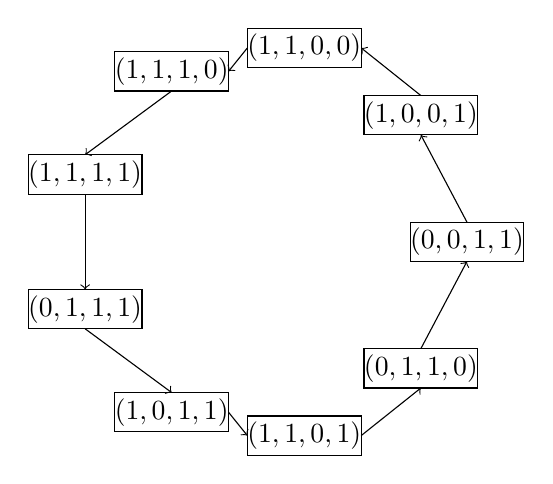
\begin{tikzpicture}[
		every node/.style = {
			draw, rectangle, 
			minimum width=0.75cm,
			minimum height=0.5cm,
			outer sep=0cm, inner sep=0cm,
			%node distance=0cm
		}
		]
		\pgfmathsetmacro\radius{2.5}
		%\draw (-4,-4) grid (4,4);
		\node (s3) at (\radius*1.0, \radius*0) {$(0, 0, 1, 1)$};
		\node (s9) at ({\radius*cos(1*2*pi/9 r)}, {\radius*sin(1*2*pi/9 r)}) {$(1, 0, 0, 1)$};
		\node (s12) at ({\radius*cos(2*2*pi/9 r)}, {\radius*sin(2*2*pi/9 r)}) {$(1, 1, 0, 0)$};
		\node (s14) at ({\radius*cos(3*2*pi/9 r)}, {\radius*sin(3*2*pi/9 r)}) {$(1, 1, 1, 0)$};
		\node (s15) at ({\radius*cos(4*2*pi/9 r)}, {\radius*sin(4*2*pi/9 r)}) {$(1, 1, 1, 1)$};
		\node (s7) at ({\radius*cos(5*2*pi/9 r)}, {\radius*sin(5*2*pi/9 r)}) {$(0, 1, 1, 1)$};
		\node (s11) at ({\radius*cos(6*2*pi/9 r)}, {\radius*sin(6*2*pi/9 r)}) {$(1, 0, 1, 1)$};
		\node (s13) at ({\radius*cos(7*2*pi/9 r)}, {\radius*sin(7*2*pi/9 r)}) {$(1, 1, 0, 1)$};
		\node (s6) at ({\radius*cos(8*2*pi/9 r)}, {\radius*sin(8*2*pi/9 r)}) {$(0, 1, 1, 0)$};
		
		\draw[->] (s3.north) -- (s9.south);
		\draw[->] (s9.north) -- (s12.east);
		\draw[->] (s12.west) -- (s14.east);
		\draw[->] (s14.south) -- (s15.north);
		\draw[->] (s15.south) -- (s7.north);
		\draw[->] (s7.south) -- (s11.north);
		\draw[->] (s11.east) -- (s13.west);
		\draw[->] (s13.east) -- (s6.south);
		\draw[->] (s6.north) -- (s3.south);
	\end{tikzpicture}
\end{document}